\documentclass[1p]{elsarticle_modified}
%\bibliographystyle{elsarticle-num}

%\usepackage[colorlinks]{hyperref}
%\usepackage{abbrmath_seonhwa} %\Abb, \Ascr, \Acal ,\Abf, \Afrak
\usepackage{amsfonts}
\usepackage{amssymb}
\usepackage{amsmath}
\usepackage{amsthm}
\usepackage{scalefnt}
\usepackage{amsbsy}
\usepackage{kotex}
\usepackage{caption}
\usepackage{subfig}
\usepackage{color}
\usepackage{graphicx}
\usepackage{xcolor} %% white, black, red, green, blue, cyan, magenta, yellow
\usepackage{float}
\usepackage{setspace}
\usepackage{hyperref}

\usepackage{tikz}
\usetikzlibrary{arrows}

\usepackage{multirow}
\usepackage{array} % fixed length table
\usepackage{hhline}

%%%%%%%%%%%%%%%%%%%%%
\makeatletter
\renewcommand*\env@matrix[1][\arraystretch]{%
	\edef\arraystretch{#1}%
	\hskip -\arraycolsep
	\let\@ifnextchar\new@ifnextchar
	\array{*\c@MaxMatrixCols c}}
\makeatother %https://tex.stackexchange.com/questions/14071/how-can-i-increase-the-line-spacing-in-a-matrix
%%%%%%%%%%%%%%%

\usepackage[normalem]{ulem}

\newcommand{\msout}[1]{\ifmmode\text{\sout{\ensuremath{#1}}}\else\sout{#1}\fi}
%SOURCE: \msout is \stkout macro in https://tex.stackexchange.com/questions/20609/strikeout-in-math-mode

\newcommand{\cancel}[1]{
	\ifmmode
	{\color{red}\msout{#1}}
	\else
	{\color{red}\sout{#1}}
	\fi
}

\newcommand{\add}[1]{
	{\color{blue}\uwave{#1}}
}

\newcommand{\replace}[2]{
	\ifmmode
	{\color{red}\msout{#1}}{\color{blue}\uwave{#2}}
	\else
	{\color{red}\sout{#1}}{\color{blue}\uwave{#2}}
	\fi
}

\newcommand{\Sol}{\mathcal{S}} %segment
\newcommand{\D}{D} %diagram
\newcommand{\A}{\mathcal{A}} %arc


%%%%%%%%%%%%%%%%%%%%%%%%%%%%%5 test

\def\sl{\operatorname{\textup{SL}}(2,\Cbb)}
\def\psl{\operatorname{\textup{PSL}}(2,\Cbb)}
\def\quan{\mkern 1mu \triangleright \mkern 1mu}

\theoremstyle{definition}
\newtheorem{thm}{Theorem}[section]
\newtheorem{prop}[thm]{Proposition}
\newtheorem{lem}[thm]{Lemma}
\newtheorem{ques}[thm]{Question}
\newtheorem{cor}[thm]{Corollary}
\newtheorem{defn}[thm]{Definition}
\newtheorem{exam}[thm]{Example}
\newtheorem{rmk}[thm]{Remark}
\newtheorem{alg}[thm]{Algorithm}

\newcommand{\I}{\sqrt{-1}}
\begin{document}

%\begin{frontmatter}
%
%\title{Boundary parabolic representations of knots up to 8 crossings}
%
%%% Group authors per affiliation:
%\author{Yunhi Cho} 
%\address{Department of Mathematics, University of Seoul, Seoul, Korea}
%\ead{yhcho@uos.ac.kr}
%
%
%\author{Seonhwa Kim} %\fnref{s_kim}}
%\address{Center for Geometry and Physics, Institute for Basic Science, Pohang, 37673, Korea}
%\ead{ryeona17@ibs.re.kr}
%
%\author{Hyuk Kim}
%\address{Department of Mathematical Sciences, Seoul National University, Seoul 08826, Korea}
%\ead{hyukkim@snu.ac.kr}
%
%\author{Seokbeom Yoon}
%\address{Department of Mathematical Sciences, Seoul National University, Seoul, 08826,  Korea}
%\ead{sbyoon15@snu.ac.kr}
%
%\begin{abstract}
%We find all boundary parabolic representation of knots up to 8 crossings.
%
%\end{abstract}
%\begin{keyword}
%    \MSC[2010] 57M25 
%\end{keyword}
%
%\end{frontmatter}

%\linenumbers
%\tableofcontents
%
\newcommand\colored[1]{\textcolor{white}{\rule[-0.35ex]{0.8em}{1.4ex}}\kern-0.8em\color{red} #1}%
%\newcommand\colored[1]{\textcolor{white}{ #1}\kern-2.17ex	\textcolor{white}{ #1}\kern-1.81ex	\textcolor{white}{ #1}\kern-2.15ex\color{red}#1	}

{\Large $\underline{12n_{0377}~(K12n_{0377})}$}

\setlength{\tabcolsep}{10pt}
\renewcommand{\arraystretch}{1.6}
\vspace{1cm}\begin{tabular}{m{100pt}>{\centering\arraybackslash}m{274pt}}
\multirow{5}{120pt}{
	\centering
	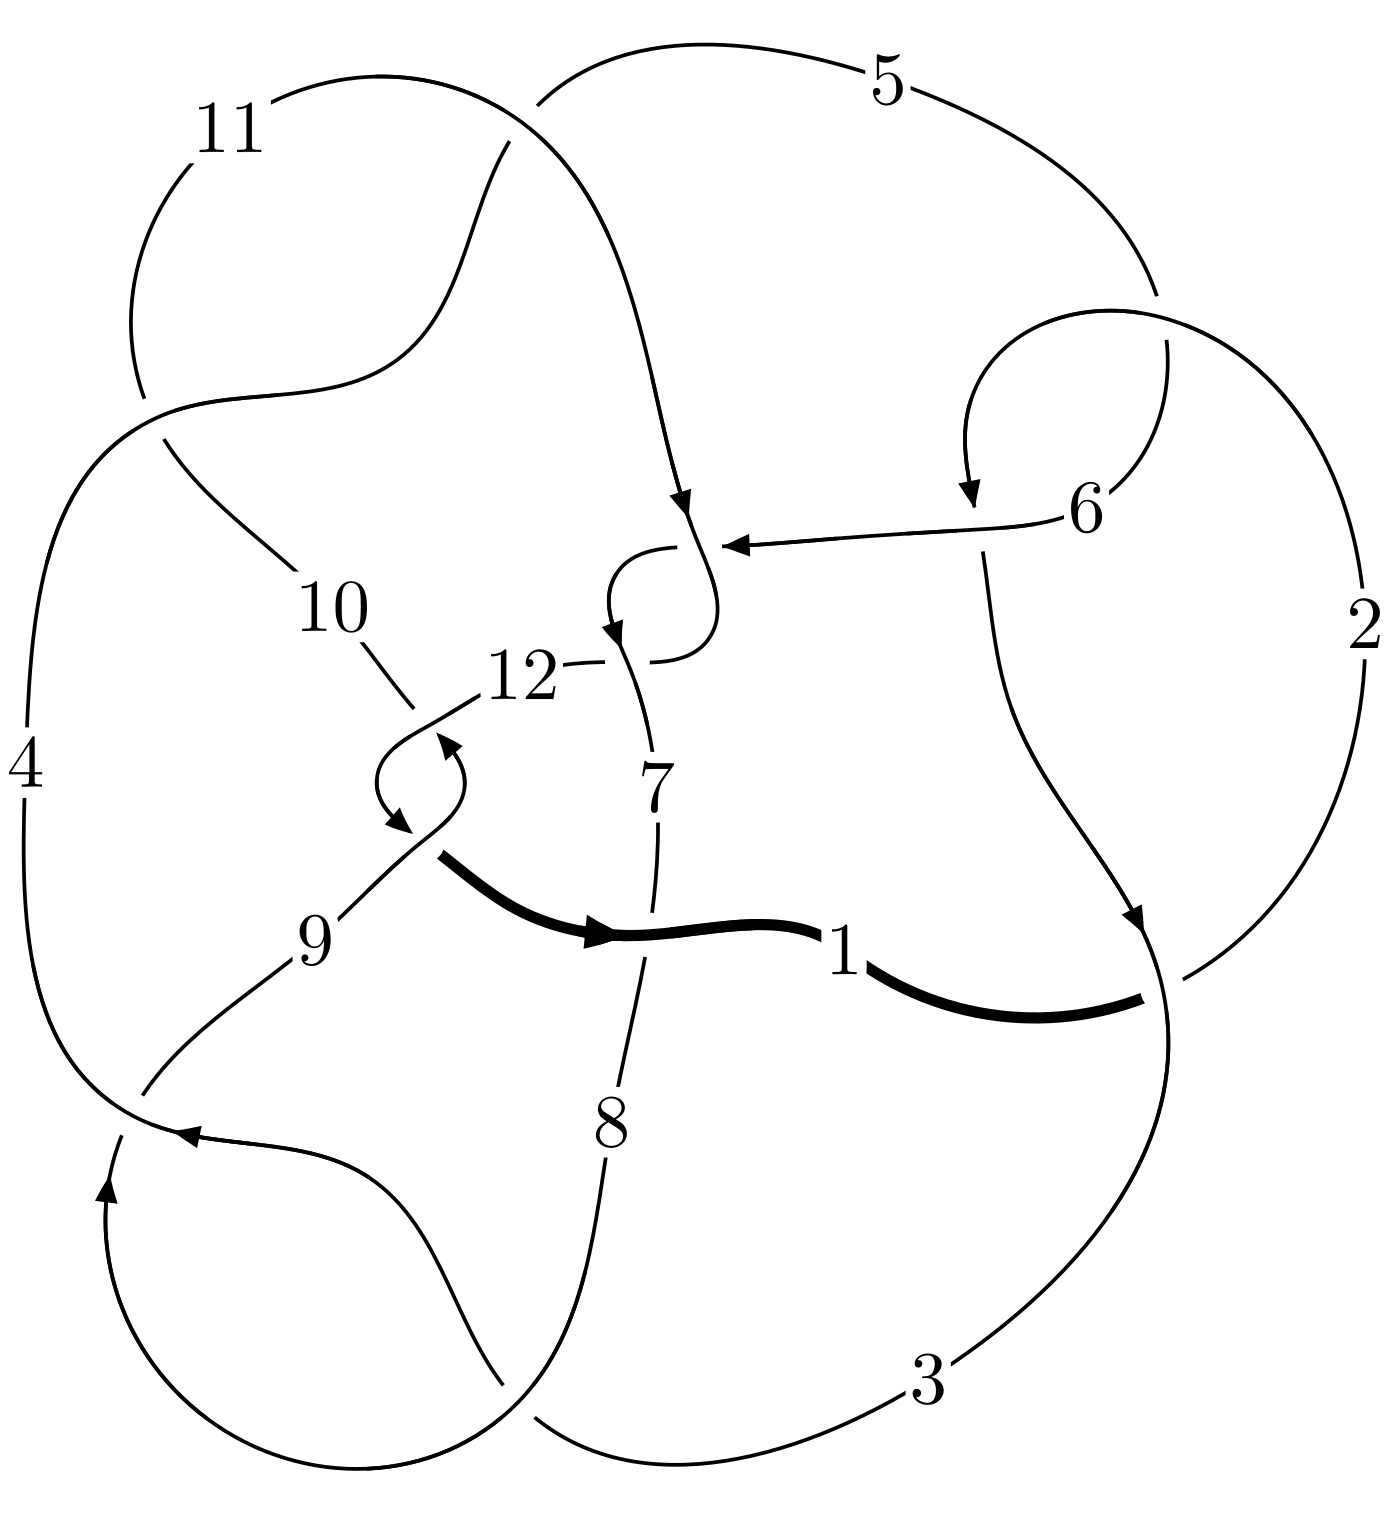
\includegraphics[width=112pt]{../../../GIT/diagram.site/Diagrams/png/2466_12n_0377.png}\\
\ \ \ A knot diagram\footnotemark}&
\allowdisplaybreaks
\textbf{Linearized knot diagam} \\
\cline{2-2}
 &
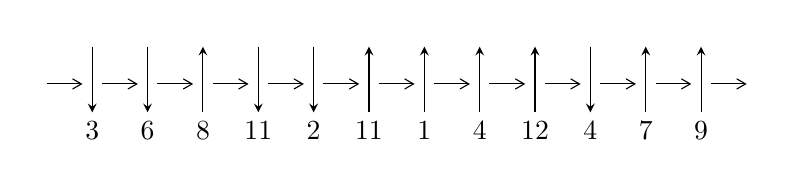
\begin{tikzpicture}[x=20pt, y=17pt]
	% nodes
	\node (C0) at (0, 0) {};
	\node (C1) at (1, 0) {};
	\node (C1U) at (1, +1) {};
	\node (C1D) at (1, -1) {3};

	\node (C2) at (2, 0) {};
	\node (C2U) at (2, +1) {};
	\node (C2D) at (2, -1) {6};

	\node (C3) at (3, 0) {};
	\node (C3U) at (3, +1) {};
	\node (C3D) at (3, -1) {8};

	\node (C4) at (4, 0) {};
	\node (C4U) at (4, +1) {};
	\node (C4D) at (4, -1) {11};

	\node (C5) at (5, 0) {};
	\node (C5U) at (5, +1) {};
	\node (C5D) at (5, -1) {2};

	\node (C6) at (6, 0) {};
	\node (C6U) at (6, +1) {};
	\node (C6D) at (6, -1) {11};

	\node (C7) at (7, 0) {};
	\node (C7U) at (7, +1) {};
	\node (C7D) at (7, -1) {1};

	\node (C8) at (8, 0) {};
	\node (C8U) at (8, +1) {};
	\node (C8D) at (8, -1) {4};

	\node (C9) at (9, 0) {};
	\node (C9U) at (9, +1) {};
	\node (C9D) at (9, -1) {12};

	\node (C10) at (10, 0) {};
	\node (C10U) at (10, +1) {};
	\node (C10D) at (10, -1) {4};

	\node (C11) at (11, 0) {};
	\node (C11U) at (11, +1) {};
	\node (C11D) at (11, -1) {7};

	\node (C12) at (12, 0) {};
	\node (C12U) at (12, +1) {};
	\node (C12D) at (12, -1) {9};
	\node (C13) at (13, 0) {};

	% arrows
	\draw[->,>={angle 60}]
	(C0) edge (C1) (C1) edge (C2) (C2) edge (C3) (C3) edge (C4) (C4) edge (C5) (C5) edge (C6) (C6) edge (C7) (C7) edge (C8) (C8) edge (C9) (C9) edge (C10) (C10) edge (C11) (C11) edge (C12) (C12) edge (C13) ;	\draw[->,>=stealth]
	(C1U) edge (C1D) (C2U) edge (C2D) (C3D) edge (C3U) (C4U) edge (C4D) (C5U) edge (C5D) (C6D) edge (C6U) (C7D) edge (C7U) (C8D) edge (C8U) (C9D) edge (C9U) (C10U) edge (C10D) (C11D) edge (C11U) (C12D) edge (C12U) ;
	\end{tikzpicture} \\
\hhline{~~} \\& 
\textbf{Solving Sequence} \\ \cline{2-2} 
 &
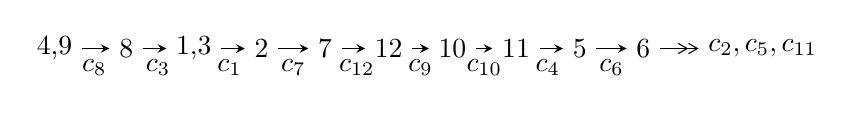
\begin{tikzpicture}[x=23pt, y=7pt]
	% node
	\node (A0) at (-1/8, 0) {4,9};
	\node (A1) at (1, 0) {8};
	\node (A2) at (33/16, 0) {1,3};
	\node (A3) at (25/8, 0) {2};
	\node (A4) at (33/8, 0) {7};
	\node (A5) at (41/8, 0) {12};
	\node (A6) at (49/8, 0) {10};
	\node (A7) at (57/8, 0) {11};
	\node (A8) at (65/8, 0) {5};
	\node (A9) at (73/8, 0) {6};
	\node (C1) at (1/2, -1) {$c_{8}$};
	\node (C2) at (3/2, -1) {$c_{3}$};
	\node (C3) at (21/8, -1) {$c_{1}$};
	\node (C4) at (29/8, -1) {$c_{7}$};
	\node (C5) at (37/8, -1) {$c_{12}$};
	\node (C6) at (45/8, -1) {$c_{9}$};
	\node (C7) at (53/8, -1) {$c_{10}$};
	\node (C8) at (61/8, -1) {$c_{4}$};
	\node (C9) at (69/8, -1) {$c_{6}$};
	\node (A10) at (11, 0) {$c_{2},c_{5},c_{11}$};

	% edge
	\draw[->,>=stealth]	
	(A0) edge (A1) (A1) edge (A2) (A2) edge (A3) (A3) edge (A4) (A4) edge (A5) (A5) edge (A6) (A6) edge (A7) (A7) edge (A8) (A8) edge (A9) ;
	\draw[->>,>={angle 60}]	
	(A9) edge (A10);
\end{tikzpicture} \\ 

\end{tabular} \\

\footnotetext{
The image of knot diagram is generated by the software ``\textbf{Draw programme}" developed by Andrew Bartholomew(\url{http://www.layer8.co.uk/maths/draw/index.htm\#Running-draw}), where we modified some parts for our purpose(\url{https://github.com/CATsTAILs/LinksPainter}).
}\phantom \\ \newline 
\centering \textbf{Ideals for irreducible components\footnotemark of $X_{\text{par}}$} 
 
\begin{align*}
I^u_{1}&=\langle 
-117109314812117 u^{21}-185021907483518 u^{20}+\cdots+71466899580913 b-239788584214052,\\
\phantom{I^u_{1}}&\phantom{= \langle  }a-1,\;u^{22}+2 u^{21}+\cdots+5 u+1\rangle \\
I^u_{2}&=\langle 
49557 u^{15}-41829 u^{14}+\cdots+54911 b+38554,\;a+1,\;u^{16}- u^{15}+\cdots+2 u+1\rangle \\
I^u_{3}&=\langle 
1927557535 u^{13}-1956930209 u^{12}+\cdots+24185780481 b-19316532454,\\
\phantom{I^u_{3}}&\phantom{= \langle  }60475263347 u^{13}+4869248027 u^{12}+\cdots+24185780481 a+118878628659,\\
\phantom{I^u_{3}}&\phantom{= \langle  }u^{14}-6 u^{12}+u^{11}-7 u^{10}+127 u^8-27 u^7-371 u^6+81 u^5+482 u^4-41 u^3-201 u^2+21 u-1\rangle \\
I^u_{4}&=\langle 
b,\;a-1,\;u-1\rangle \\
I^u_{5}&=\langle 
b,\;a- u-2,\;u^2+u-1\rangle \\
\\
\end{align*}
\raggedright * 5 irreducible components of $\dim_{\mathbb{C}}=0$, with total 55 representations.\\
\footnotetext{All coefficients of polynomials are rational numbers. But the coefficients are sometimes approximated in decimal forms when there is not enough margin.}
\newpage
\renewcommand{\arraystretch}{1}
\centering \section*{I. $I^u_{1}= \langle -1.17\times10^{14} u^{21}-1.85\times10^{14} u^{20}+\cdots+7.15\times10^{13} b-2.40\times10^{14},\;a-1,\;u^{22}+2 u^{21}+\cdots+5 u+1 \rangle$}
\flushleft \textbf{(i) Arc colorings}\\
\begin{tabular}{m{7pt} m{180pt} m{7pt} m{180pt} }
\flushright $a_{4}=$&$\begin{pmatrix}0\\u\end{pmatrix}$ \\
\flushright $a_{9}=$&$\begin{pmatrix}1\\0\end{pmatrix}$ \\
\flushright $a_{8}=$&$\begin{pmatrix}1\\u^2\end{pmatrix}$ \\
\flushright $a_{1}=$&$\begin{pmatrix}1\\1.63865 u^{21}+2.58892 u^{20}+\cdots+9.18338 u+3.35524\end{pmatrix}$ \\
\flushright $a_{3}=$&$\begin{pmatrix}- u\\- u^3+u\end{pmatrix}$ \\
\flushright $a_{2}=$&$\begin{pmatrix}-0.203702 u^{21}-0.308210 u^{20}+\cdots-1.80327 u+0.311615\\1.78179 u^{21}+2.92653 u^{20}+\cdots+10.6944 u+3.94443\end{pmatrix}$ \\
\flushright $a_{7}=$&$\begin{pmatrix}1.63865 u^{21}+2.58892 u^{20}+\cdots+9.18338 u+4.35524\\-0.810203 u^{21}-1.40823 u^{20}+\cdots-4.36829 u-3.21832\end{pmatrix}$ \\
\flushright $a_{12}=$&$\begin{pmatrix}-1.63865 u^{21}-2.58892 u^{20}+\cdots-9.18338 u-2.35524\\1.63865 u^{21}+2.58892 u^{20}+\cdots+9.18338 u+3.35524\end{pmatrix}$ \\
\flushright $a_{10}=$&$\begin{pmatrix}-2.24515 u^{21}-3.68894 u^{20}+\cdots-11.7484 u-4.88518\\0.606501 u^{21}+1.10002 u^{20}+\cdots+2.56501 u+2.52994\end{pmatrix}$ \\
\flushright $a_{11}=$&$\begin{pmatrix}-2.24515 u^{21}-3.68894 u^{20}+\cdots-11.7484 u-4.88518\\0.436584 u^{21}+0.693675 u^{20}+\cdots+0.803325 u+1.72857\end{pmatrix}$ \\
\flushright $a_{5}=$&$\begin{pmatrix}0.851249 u^{21}+1.42218 u^{20}+\cdots+7.28853 u+2.44520\\-1.23619 u^{21}-2.26646 u^{20}+\cdots-9.46092 u-3.86352\end{pmatrix}$ \\
\flushright $a_{6}=$&$\begin{pmatrix}0.573533 u^{21}+0.906242 u^{20}+\cdots+4.56014 u+1.08378\\-2.19732 u^{21}-3.69644 u^{20}+\cdots-15.9510 u-6.18859\end{pmatrix}$\\&\end{tabular}
\flushleft \textbf{(ii) Obstruction class $= -1$}\\~\\
\flushleft \textbf{(iii) Cusp Shapes $= \frac{797326516733960}{71466899580913} u^{21}+\frac{1296483474868809}{71466899580913} u^{20}+\cdots+\frac{4697397509475603}{71466899580913} u+\frac{2248576824709077}{71466899580913}$}\\~\\
\newpage\renewcommand{\arraystretch}{1}
\flushleft \textbf{(iv) u-Polynomials at the component}\newline \\
\begin{tabular}{m{50pt}|m{274pt}}
Crossings & \hspace{64pt}u-Polynomials at each crossing \\
\hline $$\begin{aligned}c_{1}\end{aligned}$$&$\begin{aligned}
&u^{22}+4 u^{21}+\cdots-126 u+25
\end{aligned}$\\
\hline $$\begin{aligned}c_{2},c_{5}\end{aligned}$$&$\begin{aligned}
&u^{22}+8 u^{21}+\cdots+12 u+5
\end{aligned}$\\
\hline $$\begin{aligned}c_{3},c_{8}\end{aligned}$$&$\begin{aligned}
&u^{22}+2 u^{21}+\cdots+5 u+1
\end{aligned}$\\
\hline $$\begin{aligned}c_{4},c_{10}\end{aligned}$$&$\begin{aligned}
&u^{22}+28 u^{20}+\cdots-2525 u+1849
\end{aligned}$\\
\hline $$\begin{aligned}c_{6},c_{11}\end{aligned}$$&$\begin{aligned}
&u^{22}+3 u^{21}+\cdots+11 u+1
\end{aligned}$\\
\hline $$\begin{aligned}c_{7}\end{aligned}$$&$\begin{aligned}
&u^{22}-15 u^{21}+\cdots-384 u+64
\end{aligned}$\\
\hline $$\begin{aligned}c_{9},c_{12}\end{aligned}$$&$\begin{aligned}
&u^{22}+11 u^{21}+\cdots+36 u+5
\end{aligned}$\\
\hline
\end{tabular}\\~\\
\newpage\renewcommand{\arraystretch}{1}
\flushleft \textbf{(v) Riley Polynomials at the component}\newline \\
\begin{tabular}{m{50pt}|m{274pt}}
Crossings & \hspace{64pt}Riley Polynomials at each crossing \\
\hline $$\begin{aligned}c_{1}\end{aligned}$$&$\begin{aligned}
&y^{22}+44 y^{21}+\cdots-15326 y+625
\end{aligned}$\\
\hline $$\begin{aligned}c_{2},c_{5}\end{aligned}$$&$\begin{aligned}
&y^{22}-4 y^{21}+\cdots+126 y+25
\end{aligned}$\\
\hline $$\begin{aligned}c_{3},c_{8}\end{aligned}$$&$\begin{aligned}
&y^{22}-26 y^{21}+\cdots-5 y+1
\end{aligned}$\\
\hline $$\begin{aligned}c_{4},c_{10}\end{aligned}$$&$\begin{aligned}
&y^{22}+56 y^{21}+\cdots-20797825 y+3418801
\end{aligned}$\\
\hline $$\begin{aligned}c_{6},c_{11}\end{aligned}$$&$\begin{aligned}
&y^{22}-39 y^{21}+\cdots+71 y+1
\end{aligned}$\\
\hline $$\begin{aligned}c_{7}\end{aligned}$$&$\begin{aligned}
&y^{22}+7 y^{21}+\cdots+32768 y+4096
\end{aligned}$\\
\hline $$\begin{aligned}c_{9},c_{12}\end{aligned}$$&$\begin{aligned}
&y^{22}+3 y^{21}+\cdots-96 y+25
\end{aligned}$\\
\hline
\end{tabular}\\~\\
\newpage\flushleft \textbf{(vi) Complex Volumes and Cusp Shapes}
$$\begin{array}{c|c|c}  
\text{Solutions to }I^u_{1}& \I (\text{vol} + \sqrt{-1}CS) & \text{Cusp shape}\\
 \hline 
\begin{aligned}
u &= -0.620794 + 0.535509 I \\
a &= \phantom{-}1.00000\phantom{ +0.000000I} \\
b &= \phantom{-}0.269144 - 0.300532 I\end{aligned}
 & -1.73171 + 0.39209 I & -6.82911 - 0.72643 I \\ \hline\begin{aligned}
u &= -0.620794 - 0.535509 I \\
a &= \phantom{-}1.00000\phantom{ +0.000000I} \\
b &= \phantom{-}0.269144 + 0.300532 I\end{aligned}
 & -1.73171 - 0.39209 I & -6.82911 + 0.72643 I \\ \hline\begin{aligned}
u &= -0.105696 + 0.706053 I \\
a &= \phantom{-}1.00000\phantom{ +0.000000I} \\
b &= -0.063961 + 0.862281 I\end{aligned}
 & -3.10436 + 1.56753 I & -1.37917 - 0.82636 I \\ \hline\begin{aligned}
u &= -0.105696 - 0.706053 I \\
a &= \phantom{-}1.00000\phantom{ +0.000000I} \\
b &= -0.063961 - 0.862281 I\end{aligned}
 & -3.10436 - 1.56753 I & -1.37917 + 0.82636 I \\ \hline\begin{aligned}
u &= \phantom{-}1.333060 + 0.198330 I \\
a &= \phantom{-}1.00000\phantom{ +0.000000I} \\
b &= \phantom{-}0.723572 - 0.172331 I\end{aligned}
 & \phantom{-}2.84189 + 0.60050 I & \phantom{-}3.92920 + 0.28556 I \\ \hline\begin{aligned}
u &= \phantom{-}1.333060 - 0.198330 I \\
a &= \phantom{-}1.00000\phantom{ +0.000000I} \\
b &= \phantom{-}0.723572 + 0.172331 I\end{aligned}
 & \phantom{-}2.84189 - 0.60050 I & \phantom{-}3.92920 - 0.28556 I \\ \hline\begin{aligned}
u &= -0.056495 + 0.552181 I \\
a &= \phantom{-}1.00000\phantom{ +0.000000I} \\
b &= -0.487168 - 1.034230 I\end{aligned}
 & -0.79249 + 2.57985 I & \phantom{-}0.76440 - 3.56435 I \\ \hline\begin{aligned}
u &= -0.056495 - 0.552181 I \\
a &= \phantom{-}1.00000\phantom{ +0.000000I} \\
b &= -0.487168 + 1.034230 I\end{aligned}
 & -0.79249 - 2.57985 I & \phantom{-}0.76440 + 3.56435 I \\ \hline\begin{aligned}
u &= -1.41493 + 0.47947 I \\
a &= \phantom{-}1.00000\phantom{ +0.000000I} \\
b &= \phantom{-}0.921745 - 0.224366 I\end{aligned}
 & \phantom{-}1.50957 - 6.23042 I & \phantom{-}2.89462 + 2.84257 I \\ \hline\begin{aligned}
u &= -1.41493 - 0.47947 I \\
a &= \phantom{-}1.00000\phantom{ +0.000000I} \\
b &= \phantom{-}0.921745 + 0.224366 I\end{aligned}
 & \phantom{-}1.50957 + 6.23042 I & \phantom{-}2.89462 - 2.84257 I\\
 \hline 
 \end{array}$$\newpage$$\begin{array}{c|c|c}  
\text{Solutions to }I^u_{1}& \I (\text{vol} + \sqrt{-1}CS) & \text{Cusp shape}\\
 \hline 
\begin{aligned}
u &= \phantom{-}0.290445 + 0.380257 I \\
a &= \phantom{-}1.00000\phantom{ +0.000000I} \\
b &= -0.658679 - 0.004198 I\end{aligned}
 & \phantom{-}1.41421 + 0.48473 I & \phantom{-}7.29881 - 2.06718 I \\ \hline\begin{aligned}
u &= \phantom{-}0.290445 - 0.380257 I \\
a &= \phantom{-}1.00000\phantom{ +0.000000I} \\
b &= -0.658679 + 0.004198 I\end{aligned}
 & \phantom{-}1.41421 - 0.48473 I & \phantom{-}7.29881 + 2.06718 I \\ \hline\begin{aligned}
u &= \phantom{-}1.52781 + 0.03204 I \\
a &= \phantom{-}1.00000\phantom{ +0.000000I} \\
b &= \phantom{-}1.09000 - 1.35357 I\end{aligned}
 & \phantom{-}15.9443 - 3.5566 I & \phantom{-}4.85061 + 2.05487 I \\ \hline\begin{aligned}
u &= \phantom{-}1.52781 - 0.03204 I \\
a &= \phantom{-}1.00000\phantom{ +0.000000I} \\
b &= \phantom{-}1.09000 + 1.35357 I\end{aligned}
 & \phantom{-}15.9443 + 3.5566 I & \phantom{-}4.85061 - 2.05487 I \\ \hline\begin{aligned}
u &= -1.58478 + 0.02890 I \\
a &= \phantom{-}1.00000\phantom{ +0.000000I} \\
b &= \phantom{-}1.25856 + 1.26328 I\end{aligned}
 & \phantom{-}16.5982 - 4.1754 I & \phantom{-}5.36851 + 2.13460 I \\ \hline\begin{aligned}
u &= -1.58478 - 0.02890 I \\
a &= \phantom{-}1.00000\phantom{ +0.000000I} \\
b &= \phantom{-}1.25856 - 1.26328 I\end{aligned}
 & \phantom{-}16.5982 + 4.1754 I & \phantom{-}5.36851 - 2.13460 I \\ \hline\begin{aligned}
u &= -0.369059 + 0.081714 I \\
a &= \phantom{-}1.00000\phantom{ +0.000000I} \\
b &= -0.113829 + 1.356110 I\end{aligned}
 & -3.96081 - 3.52484 I & \phantom{-}7.30433 + 8.96045 I \\ \hline\begin{aligned}
u &= -0.369059 - 0.081714 I \\
a &= \phantom{-}1.00000\phantom{ +0.000000I} \\
b &= -0.113829 - 1.356110 I\end{aligned}
 & -3.96081 + 3.52484 I & \phantom{-}7.30433 - 8.96045 I \\ \hline\begin{aligned}
u &= \phantom{-}1.74996 + 0.63959 I \\
a &= \phantom{-}1.00000\phantom{ +0.000000I} \\
b &= \phantom{-}1.32824 + 1.03454 I\end{aligned}
 & \phantom{-}17.0359 + 5.3783 I & \phantom{-}5.15920 - 2.10879 I \\ \hline\begin{aligned}
u &= \phantom{-}1.74996 - 0.63959 I \\
a &= \phantom{-}1.00000\phantom{ +0.000000I} \\
b &= \phantom{-}1.32824 - 1.03454 I\end{aligned}
 & \phantom{-}17.0359 - 5.3783 I & \phantom{-}5.15920 + 2.10879 I\\
 \hline 
 \end{array}$$\newpage$$\begin{array}{c|c|c}  
\text{Solutions to }I^u_{1}& \I (\text{vol} + \sqrt{-1}CS) & \text{Cusp shape}\\
 \hline 
\begin{aligned}
u &= -1.74953 + 0.66838 I \\
a &= \phantom{-}1.00000\phantom{ +0.000000I} \\
b &= \phantom{-}1.23238 - 1.16964 I\end{aligned}
 & \phantom{-}16.7528 - 13.3075 I & \phantom{-}4.63861 + 6.01533 I \\ \hline\begin{aligned}
u &= -1.74953 - 0.66838 I \\
a &= \phantom{-}1.00000\phantom{ +0.000000I} \\
b &= \phantom{-}1.23238 + 1.16964 I\end{aligned}
 & \phantom{-}16.7528 + 13.3075 I & \phantom{-}4.63861 - 6.01533 I\\
 \hline 
 \end{array}$$\newpage\newpage\renewcommand{\arraystretch}{1}
\centering \section*{II. $I^u_{2}= \langle 49557 u^{15}-41829 u^{14}+\cdots+54911 b+38554,\;a+1,\;u^{16}- u^{15}+\cdots+2 u+1 \rangle$}
\flushleft \textbf{(i) Arc colorings}\\
\begin{tabular}{m{7pt} m{180pt} m{7pt} m{180pt} }
\flushright $a_{4}=$&$\begin{pmatrix}0\\u\end{pmatrix}$ \\
\flushright $a_{9}=$&$\begin{pmatrix}1\\0\end{pmatrix}$ \\
\flushright $a_{8}=$&$\begin{pmatrix}1\\u^2\end{pmatrix}$ \\
\flushright $a_{1}=$&$\begin{pmatrix}-1\\-0.902497 u^{15}+0.761760 u^{14}+\cdots-1.46801 u-0.702118\end{pmatrix}$ \\
\flushright $a_{3}=$&$\begin{pmatrix}- u\\- u^3+u\end{pmatrix}$ \\
\flushright $a_{2}=$&$\begin{pmatrix}0.370636 u^{15}-0.375917 u^{14}+\cdots-1.18397 u-1.14074\\-0.914371 u^{15}+0.649196 u^{14}+\cdots-0.644115 u-0.556100\end{pmatrix}$ \\
\flushright $a_{7}=$&$\begin{pmatrix}0.902497 u^{15}-0.761760 u^{14}+\cdots+1.46801 u+1.70212\\0.217570 u^{15}-0.135273 u^{14}+\cdots+1.32194 u-1.08969\end{pmatrix}$ \\
\flushright $a_{12}=$&$\begin{pmatrix}0.902497 u^{15}-0.761760 u^{14}+\cdots+1.46801 u-0.297882\\-0.902497 u^{15}+0.761760 u^{14}+\cdots-1.46801 u-0.702118\end{pmatrix}$ \\
\flushright $a_{10}=$&$\begin{pmatrix}-0.314290 u^{15}+0.250569 u^{14}+\cdots-1.33004 u-0.932545\\-0.588206 u^{15}+0.511191 u^{14}+\cdots-0.137969 u+1.23043\end{pmatrix}$ \\
\flushright $a_{11}=$&$\begin{pmatrix}-0.314290 u^{15}+0.250569 u^{14}+\cdots-1.33004 u-0.932545\\-0.880243 u^{15}+0.779480 u^{14}+\cdots+0.303764 u+1.29415\end{pmatrix}$ \\
\flushright $a_{5}=$&$\begin{pmatrix}-0.110615 u^{15}-0.168272 u^{14}+\cdots+0.347162 u+0.575021\\-0.320883 u^{15}-0.226038 u^{14}+\cdots+4.37586 u+0.584109\end{pmatrix}$ \\
\flushright $a_{6}=$&$\begin{pmatrix}0.327475 u^{15}-0.297354 u^{14}+\cdots-1.08177 u+0.899237\\-0.366539 u^{15}+0.127953 u^{14}+\cdots+4.97174 u+1.11795\end{pmatrix}$\\&\end{tabular}
\flushleft \textbf{(ii) Obstruction class $= 1$}\\~\\
\flushleft \textbf{(iii) Cusp Shapes $= \frac{57612}{54911} u^{15}-\frac{210798}{54911} u^{14}+\cdots+\frac{882421}{54911} u+\frac{37697}{54911}$}\\~\\
\newpage\renewcommand{\arraystretch}{1}
\flushleft \textbf{(iv) u-Polynomials at the component}\newline \\
\begin{tabular}{m{50pt}|m{274pt}}
Crossings & \hspace{64pt}u-Polynomials at each crossing \\
\hline $$\begin{aligned}c_{1}\end{aligned}$$&$\begin{aligned}
&u^{16}-5 u^{15}+\cdots-9 u+1
\end{aligned}$\\
\hline $$\begin{aligned}c_{2}\end{aligned}$$&$\begin{aligned}
&u^{16}+5 u^{15}+\cdots+5 u+1
\end{aligned}$\\
\hline $$\begin{aligned}c_{3}\end{aligned}$$&$\begin{aligned}
&u^{16}+u^{15}+\cdots-2 u+1
\end{aligned}$\\
\hline $$\begin{aligned}c_{4}\end{aligned}$$&$\begin{aligned}
&u^{16}- u^{15}+\cdots+2 u+1
\end{aligned}$\\
\hline $$\begin{aligned}c_{5}\end{aligned}$$&$\begin{aligned}
&u^{16}-5 u^{15}+\cdots-5 u+1
\end{aligned}$\\
\hline $$\begin{aligned}c_{6}\end{aligned}$$&$\begin{aligned}
&u^{16}+2 u^{15}+\cdots+2 u+1
\end{aligned}$\\
\hline $$\begin{aligned}c_{7}\end{aligned}$$&$\begin{aligned}
&u^{16}-3 u^{15}+\cdots- u+1
\end{aligned}$\\
\hline $$\begin{aligned}c_{8}\end{aligned}$$&$\begin{aligned}
&u^{16}- u^{15}+\cdots+2 u+1
\end{aligned}$\\
\hline $$\begin{aligned}c_{9}\end{aligned}$$&$\begin{aligned}
&u^{16}+8 u^{15}+\cdots+23 u+5
\end{aligned}$\\
\hline $$\begin{aligned}c_{10}\end{aligned}$$&$\begin{aligned}
&u^{16}+u^{15}+\cdots-2 u+1
\end{aligned}$\\
\hline $$\begin{aligned}c_{11}\end{aligned}$$&$\begin{aligned}
&u^{16}-2 u^{15}+\cdots-2 u+1
\end{aligned}$\\
\hline $$\begin{aligned}c_{12}\end{aligned}$$&$\begin{aligned}
&u^{16}-8 u^{15}+\cdots-23 u+5
\end{aligned}$\\
\hline
\end{tabular}\\~\\
\newpage\renewcommand{\arraystretch}{1}
\flushleft \textbf{(v) Riley Polynomials at the component}\newline \\
\begin{tabular}{m{50pt}|m{274pt}}
Crossings & \hspace{64pt}Riley Polynomials at each crossing \\
\hline $$\begin{aligned}c_{1}\end{aligned}$$&$\begin{aligned}
&y^{16}+11 y^{15}+\cdots-9 y+1
\end{aligned}$\\
\hline $$\begin{aligned}c_{2},c_{5}\end{aligned}$$&$\begin{aligned}
&y^{16}-5 y^{15}+\cdots-9 y+1
\end{aligned}$\\
\hline $$\begin{aligned}c_{3},c_{8}\end{aligned}$$&$\begin{aligned}
&y^{16}-11 y^{15}+\cdots+4 y+1
\end{aligned}$\\
\hline $$\begin{aligned}c_{4},c_{10}\end{aligned}$$&$\begin{aligned}
&y^{16}+15 y^{15}+\cdots-8 y+1
\end{aligned}$\\
\hline $$\begin{aligned}c_{6},c_{11}\end{aligned}$$&$\begin{aligned}
&y^{16}-12 y^{15}+\cdots-4 y+1
\end{aligned}$\\
\hline $$\begin{aligned}c_{7}\end{aligned}$$&$\begin{aligned}
&y^{16}+7 y^{15}+\cdots-5 y+1
\end{aligned}$\\
\hline $$\begin{aligned}c_{9},c_{12}\end{aligned}$$&$\begin{aligned}
&y^{16}+6 y^{15}+\cdots-139 y+25
\end{aligned}$\\
\hline
\end{tabular}\\~\\
\newpage\flushleft \textbf{(vi) Complex Volumes and Cusp Shapes}
$$\begin{array}{c|c|c}  
\text{Solutions to }I^u_{2}& \I (\text{vol} + \sqrt{-1}CS) & \text{Cusp shape}\\
 \hline 
\begin{aligned}
u &= -0.954777 + 0.142609 I \\
a &= -1.00000\phantom{ +0.000000I} \\
b &= -0.455945 - 1.267540 I\end{aligned}
 & -0.95352 - 2.33937 I & \phantom{-}3.69928 + 2.27145 I \\ \hline\begin{aligned}
u &= -0.954777 - 0.142609 I \\
a &= -1.00000\phantom{ +0.000000I} \\
b &= -0.455945 + 1.267540 I\end{aligned}
 & -0.95352 + 2.33937 I & \phantom{-}3.69928 - 2.27145 I \\ \hline\begin{aligned}
u &= \phantom{-}0.845388 + 0.160874 I \\
a &= -1.00000\phantom{ +0.000000I} \\
b &= -0.42793 - 1.42727 I\end{aligned}
 & \phantom{-}0.65993 + 3.36157 I & \phantom{-}4.55859 - 4.29560 I \\ \hline\begin{aligned}
u &= \phantom{-}0.845388 - 0.160874 I \\
a &= -1.00000\phantom{ +0.000000I} \\
b &= -0.42793 + 1.42727 I\end{aligned}
 & \phantom{-}0.65993 - 3.36157 I & \phantom{-}4.55859 + 4.29560 I \\ \hline\begin{aligned}
u &= -0.661594 + 0.474483 I \\
a &= -1.00000\phantom{ +0.000000I} \\
b &= -0.654799 + 0.242436 I\end{aligned}
 & -0.903865 + 0.284978 I & \phantom{-}4.15730 + 0.76962 I \\ \hline\begin{aligned}
u &= -0.661594 - 0.474483 I \\
a &= -1.00000\phantom{ +0.000000I} \\
b &= -0.654799 - 0.242436 I\end{aligned}
 & -0.903865 - 0.284978 I & \phantom{-}4.15730 - 0.76962 I \\ \hline\begin{aligned}
u &= -0.030530 + 1.200850 I \\
a &= -1.00000\phantom{ +0.000000I} \\
b &= \phantom{-}0.643145 + 0.122983 I\end{aligned}
 & \phantom{-}9.47497 + 3.82028 I & \phantom{-}0.82572 - 2.11435 I \\ \hline\begin{aligned}
u &= -0.030530 - 1.200850 I \\
a &= -1.00000\phantom{ +0.000000I} \\
b &= \phantom{-}0.643145 - 0.122983 I\end{aligned}
 & \phantom{-}9.47497 - 3.82028 I & \phantom{-}0.82572 + 2.11435 I \\ \hline\begin{aligned}
u &= \phantom{-}1.329520 + 0.350471 I \\
a &= -1.00000\phantom{ +0.000000I} \\
b &= -1.140330 - 0.634965 I\end{aligned}
 & \phantom{-}3.99670 + 2.81389 I & \phantom{-}5.17513 - 2.85413 I \\ \hline\begin{aligned}
u &= \phantom{-}1.329520 - 0.350471 I \\
a &= -1.00000\phantom{ +0.000000I} \\
b &= -1.140330 + 0.634965 I\end{aligned}
 & \phantom{-}3.99670 - 2.81389 I & \phantom{-}5.17513 + 2.85413 I\\
 \hline 
 \end{array}$$\newpage$$\begin{array}{c|c|c}  
\text{Solutions to }I^u_{2}& \I (\text{vol} + \sqrt{-1}CS) & \text{Cusp shape}\\
 \hline 
\begin{aligned}
u &= -1.38404 + 0.60477 I \\
a &= -1.00000\phantom{ +0.000000I} \\
b &= -0.826464 + 0.694550 I\end{aligned}
 & \phantom{-}1.21063 - 7.51551 I & \phantom{-}0.30224 + 8.63073 I \\ \hline\begin{aligned}
u &= -1.38404 - 0.60477 I \\
a &= -1.00000\phantom{ +0.000000I} \\
b &= -0.826464 - 0.694550 I\end{aligned}
 & \phantom{-}1.21063 + 7.51551 I & \phantom{-}0.30224 - 8.63073 I \\ \hline\begin{aligned}
u &= \phantom{-}1.48217 + 0.35127 I \\
a &= -1.00000\phantom{ +0.000000I} \\
b &= -0.941782 - 0.971401 I\end{aligned}
 & \phantom{-}3.96834 + 3.49267 I & \phantom{-}6.27073 - 2.05893 I \\ \hline\begin{aligned}
u &= \phantom{-}1.48217 - 0.35127 I \\
a &= -1.00000\phantom{ +0.000000I} \\
b &= -0.941782 + 0.971401 I\end{aligned}
 & \phantom{-}3.96834 - 3.49267 I & \phantom{-}6.27073 + 2.05893 I \\ \hline\begin{aligned}
u &= -0.126135 + 0.368078 I \\
a &= -1.00000\phantom{ +0.000000I} \\
b &= -0.195896 - 1.263040 I\end{aligned}
 & -4.29370 + 3.24685 I & -6.98898 + 1.98047 I \\ \hline\begin{aligned}
u &= -0.126135 - 0.368078 I \\
a &= -1.00000\phantom{ +0.000000I} \\
b &= -0.195896 + 1.263040 I\end{aligned}
 & -4.29370 - 3.24685 I & -6.98898 - 1.98047 I\\
 \hline 
 \end{array}$$\newpage\newpage\renewcommand{\arraystretch}{1}
\centering \section*{III. $I^u_{3}= \langle 1.93\times10^{9} u^{13}-1.96\times10^{9} u^{12}+\cdots+2.42\times10^{10} b-1.93\times10^{10},\;6.05\times10^{10} u^{13}+4.87\times10^{9} u^{12}+\cdots+2.42\times10^{10} a+1.19\times10^{11},\;u^{14}-6 u^{12}+\cdots+21 u-1 \rangle$}
\flushleft \textbf{(i) Arc colorings}\\
\begin{tabular}{m{7pt} m{180pt} m{7pt} m{180pt} }
\flushright $a_{4}=$&$\begin{pmatrix}0\\u\end{pmatrix}$ \\
\flushright $a_{9}=$&$\begin{pmatrix}1\\0\end{pmatrix}$ \\
\flushright $a_{8}=$&$\begin{pmatrix}1\\u^2\end{pmatrix}$ \\
\flushright $a_{1}=$&$\begin{pmatrix}-2.50045 u^{13}-0.201327 u^{12}+\cdots+498.185 u-4.91523\\-0.0796980 u^{13}+0.0809124 u^{12}+\cdots+1.72742 u+0.798673\end{pmatrix}$ \\
\flushright $a_{3}=$&$\begin{pmatrix}- u\\- u^3+u\end{pmatrix}$ \\
\flushright $a_{2}=$&$\begin{pmatrix}-2.42075 u^{13}-0.282239 u^{12}+\cdots+496.457 u-4.71390\\-0.0369901 u^{13}+0.00188849 u^{12}+\cdots+5.23369 u+0.516434\end{pmatrix}$ \\
\flushright $a_{7}=$&$\begin{pmatrix}-2.50045 u^{13}-0.201327 u^{12}+\cdots+498.185 u-3.91523\\-0.0796980 u^{13}+0.0809124 u^{12}+\cdots+1.72742 u+0.798673\end{pmatrix}$ \\
\flushright $a_{12}=$&$\begin{pmatrix}-2.42075 u^{13}-0.282239 u^{12}+\cdots+496.457 u-5.71390\\-0.0796980 u^{13}+0.0809124 u^{12}+\cdots+1.72742 u+0.798673\end{pmatrix}$ \\
\flushright $a_{10}=$&$\begin{pmatrix}2.45112 u^{13}+0.157103 u^{12}+\cdots-490.012 u+11.1679\\-0.137834 u^{13}+0.206995 u^{12}+\cdots-7.06018 u-0.434576\end{pmatrix}$ \\
\flushright $a_{11}=$&$\begin{pmatrix}2.45112 u^{13}+0.157103 u^{12}+\cdots-490.012 u+11.1679\\-0.0855064 u^{13}+0.157616 u^{12}+\cdots-7.90821 u-0.277473\end{pmatrix}$ \\
\flushright $a_{5}=$&$\begin{pmatrix}1.90624 u^{13}-0.119682 u^{12}+\cdots-392.906 u+68.8828\\0.0998596 u^{13}+0.0125182 u^{12}+\cdots-24.2787 u+2.08825\end{pmatrix}$ \\
\flushright $a_{6}=$&$\begin{pmatrix}2.12010 u^{13}+0.153572 u^{12}+\cdots-440.511 u+24.1292\\0.00222918 u^{13}+0.0614998 u^{12}+\cdots-12.0319 u+0.363834\end{pmatrix}$\\&\end{tabular}
\flushleft \textbf{(ii) Obstruction class $= -1$}\\~\\
\flushleft \textbf{(iii) Cusp Shapes $= \frac{6739667375}{24185780481} u^{13}+\frac{3644507297}{24185780481} u^{12}+\cdots-\frac{1559248921091}{24185780481} u+\frac{342583935034}{24185780481}$}\\~\\
\newpage\renewcommand{\arraystretch}{1}
\flushleft \textbf{(iv) u-Polynomials at the component}\newline \\
\begin{tabular}{m{50pt}|m{274pt}}
Crossings & \hspace{64pt}u-Polynomials at each crossing \\
\hline $$\begin{aligned}c_{1}\end{aligned}$$&$\begin{aligned}
&(u^7+4 u^5+u^4-6 u^3+3 u^2-2 u+1)^2
\end{aligned}$\\
\hline $$\begin{aligned}c_{2},c_{5}\end{aligned}$$&$\begin{aligned}
&(u^7-2 u^6+2 u^5+u^4-2 u^3+3 u^2-2 u+1)^2
\end{aligned}$\\
\hline $$\begin{aligned}c_{3},c_{8}\end{aligned}$$&$\begin{aligned}
&u^{14}-6 u^{12}+\cdots+21 u-1
\end{aligned}$\\
\hline $$\begin{aligned}c_{4},c_{10}\end{aligned}$$&$\begin{aligned}
&u^{14}+2 u^{13}+\cdots+2543 u+563
\end{aligned}$\\
\hline $$\begin{aligned}c_{6},c_{11}\end{aligned}$$&$\begin{aligned}
&u^{14}-3 u^{13}+\cdots-666 u-297
\end{aligned}$\\
\hline $$\begin{aligned}c_{7}\end{aligned}$$&$\begin{aligned}
&(u+1)^{14}
\end{aligned}$\\
\hline $$\begin{aligned}c_{9},c_{12}\end{aligned}$$&$\begin{aligned}
&(u^7-3 u^6+3 u^5+2 u^4-6 u^3+3 u^2+3 u-2)^2
\end{aligned}$\\
\hline
\end{tabular}\\~\\
\newpage\renewcommand{\arraystretch}{1}
\flushleft \textbf{(v) Riley Polynomials at the component}\newline \\
\begin{tabular}{m{50pt}|m{274pt}}
Crossings & \hspace{64pt}Riley Polynomials at each crossing \\
\hline $$\begin{aligned}c_{1}\end{aligned}$$&$\begin{aligned}
&(y^7+8 y^6+4 y^5-53 y^4+14 y^3+13 y^2-2 y-1)^2
\end{aligned}$\\
\hline $$\begin{aligned}c_{2},c_{5}\end{aligned}$$&$\begin{aligned}
&(y^7+4 y^5- y^4-6 y^3-3 y^2-2 y-1)^2
\end{aligned}$\\
\hline $$\begin{aligned}c_{3},c_{8}\end{aligned}$$&$\begin{aligned}
&y^{14}-12 y^{13}+\cdots-39 y+1
\end{aligned}$\\
\hline $$\begin{aligned}c_{4},c_{10}\end{aligned}$$&$\begin{aligned}
&y^{14}+36 y^{13}+\cdots-1927943 y+316969
\end{aligned}$\\
\hline $$\begin{aligned}c_{6},c_{11}\end{aligned}$$&$\begin{aligned}
&y^{14}-23 y^{13}+\cdots-641358 y+88209
\end{aligned}$\\
\hline $$\begin{aligned}c_{7}\end{aligned}$$&$\begin{aligned}
&(y-1)^{14}
\end{aligned}$\\
\hline $$\begin{aligned}c_{9},c_{12}\end{aligned}$$&$\begin{aligned}
&(y^7-3 y^6+9 y^5-16 y^4+30 y^3-37 y^2+21 y-4)^2
\end{aligned}$\\
\hline
\end{tabular}\\~\\
\newpage\flushleft \textbf{(vi) Complex Volumes and Cusp Shapes}
$$\begin{array}{c|c|c}  
\text{Solutions to }I^u_{3}& \I (\text{vol} + \sqrt{-1}CS) & \text{Cusp shape}\\
 \hline 
\begin{aligned}
u &= -1.215940 + 0.220023 I \\
a &= -1.54528 - 0.08333 I \\
b &= -1.25449 + 0.70767 I\end{aligned}
 & \phantom{-}5.41964 - 2.53884 I & \phantom{-}12.86344 + 1.81085 I \\ \hline\begin{aligned}
u &= -1.215940 - 0.220023 I \\
a &= -1.54528 + 0.08333 I \\
b &= -1.25449 - 0.70767 I\end{aligned}
 & \phantom{-}5.41964 + 2.53884 I & \phantom{-}12.86344 - 1.81085 I \\ \hline\begin{aligned}
u &= \phantom{-}0.758211\phantom{ +0.000000I} \\
a &= -2.80601\phantom{ +0.000000I} \\
b &= -0.613130\phantom{ +0.000000I}\end{aligned}
 & \phantom{-}0.459094\phantom{ +0.000000I} & \phantom{-}13.7190\phantom{ +0.000000I} \\ \hline\begin{aligned}
u &= -1.400900 + 0.122011 I \\
a &= -1.010470 + 0.394732 I \\
b &= -0.833081 + 1.114220 I\end{aligned}
 & \phantom{-}3.62587 - 4.72329 I & \phantom{-}4.98093 + 9.17288 I \\ \hline\begin{aligned}
u &= -1.400900 - 0.122011 I \\
a &= -1.010470 - 0.394732 I \\
b &= -0.833081 - 1.114220 I\end{aligned}
 & \phantom{-}3.62587 + 4.72329 I & \phantom{-}4.98093 - 9.17288 I \\ \hline\begin{aligned}
u &= \phantom{-}1.36740 + 0.67627 I \\
a &= -0.858613 + 0.335410 I \\
b &= -0.833081 - 1.114220 I\end{aligned}
 & \phantom{-}3.62587 + 4.72329 I & \phantom{-}4.98093 - 9.17288 I \\ \hline\begin{aligned}
u &= \phantom{-}1.36740 - 0.67627 I \\
a &= -0.858613 - 0.335410 I \\
b &= -0.833081 + 1.114220 I\end{aligned}
 & \phantom{-}3.62587 - 4.72329 I & \phantom{-}4.98093 + 9.17288 I \\ \hline\begin{aligned}
u &= \phantom{-}1.89730 + 0.23868 I \\
a &= -0.645256 - 0.034794 I \\
b &= -1.25449 - 0.70767 I\end{aligned}
 & \phantom{-}5.41964 + 2.53884 I & \phantom{-}12.86344 - 1.81085 I \\ \hline\begin{aligned}
u &= \phantom{-}1.89730 - 0.23868 I \\
a &= -0.645256 + 0.034794 I \\
b &= -1.25449 + 0.70767 I\end{aligned}
 & \phantom{-}5.41964 - 2.53884 I & \phantom{-}12.86344 + 1.81085 I \\ \hline\begin{aligned}
u &= \phantom{-}0.0517518 + 0.0475534 I \\
a &= \phantom{-}21.1195 + 23.2984 I \\
b &= \phantom{-}0.894131 + 0.113662 I\end{aligned}
 & \phantom{-}10.46420 + 3.91715 I & \phantom{-}10.79602 - 3.00324 I\\
 \hline 
 \end{array}$$\newpage$$\begin{array}{c|c|c}  
\text{Solutions to }I^u_{3}& \I (\text{vol} + \sqrt{-1}CS) & \text{Cusp shape}\\
 \hline 
\begin{aligned}
u &= \phantom{-}0.0517518 - 0.0475534 I \\
a &= \phantom{-}21.1195 - 23.2984 I \\
b &= \phantom{-}0.894131 - 0.113662 I\end{aligned}
 & \phantom{-}10.46420 - 3.91715 I & \phantom{-}10.79602 + 3.00324 I \\ \hline\begin{aligned}
u &= -2.12755\phantom{ +0.000000I} \\
a &= -0.356378\phantom{ +0.000000I} \\
b &= -0.613130\phantom{ +0.000000I}\end{aligned}
 & \phantom{-}0.459094\phantom{ +0.000000I} & \phantom{-}13.7190\phantom{ +0.000000I} \\ \hline\begin{aligned}
u &= -0.01495 + 2.21004 I \\
a &= \phantom{-}0.0213576 - 0.0235612 I \\
b &= \phantom{-}0.894131 + 0.113662 I\end{aligned}
 & \phantom{-}10.46420 + 3.91715 I & \phantom{-}10.79602 - 3.00324 I \\ \hline\begin{aligned}
u &= -0.01495 - 2.21004 I \\
a &= \phantom{-}0.0213576 + 0.0235612 I \\
b &= \phantom{-}0.894131 - 0.113662 I\end{aligned}
 & \phantom{-}10.46420 - 3.91715 I & \phantom{-}10.79602 + 3.00324 I\\
 \hline 
 \end{array}$$\newpage\newpage\renewcommand{\arraystretch}{1}
\centering \section*{IV. $I^u_{4}= \langle b,\;a-1,\;u-1 \rangle$}
\flushleft \textbf{(i) Arc colorings}\\
\begin{tabular}{m{7pt} m{180pt} m{7pt} m{180pt} }
\flushright $a_{4}=$&$\begin{pmatrix}0\\1\end{pmatrix}$ \\
\flushright $a_{9}=$&$\begin{pmatrix}1\\0\end{pmatrix}$ \\
\flushright $a_{8}=$&$\begin{pmatrix}1\\1\end{pmatrix}$ \\
\flushright $a_{1}=$&$\begin{pmatrix}1\\0\end{pmatrix}$ \\
\flushright $a_{3}=$&$\begin{pmatrix}-1\\0\end{pmatrix}$ \\
\flushright $a_{2}=$&$\begin{pmatrix}1\\0\end{pmatrix}$ \\
\flushright $a_{7}=$&$\begin{pmatrix}0\\1\end{pmatrix}$ \\
\flushright $a_{12}=$&$\begin{pmatrix}1\\0\end{pmatrix}$ \\
\flushright $a_{10}=$&$\begin{pmatrix}1\\0\end{pmatrix}$ \\
\flushright $a_{11}=$&$\begin{pmatrix}1\\1\end{pmatrix}$ \\
\flushright $a_{5}=$&$\begin{pmatrix}-1\\0\end{pmatrix}$ \\
\flushright $a_{6}=$&$\begin{pmatrix}-1\\0\end{pmatrix}$\\&\end{tabular}
\flushleft \textbf{(ii) Obstruction class $= -1$}\\~\\
\flushleft \textbf{(iii) Cusp Shapes $= 6$}\\~\\
\newpage\renewcommand{\arraystretch}{1}
\flushleft \textbf{(iv) u-Polynomials at the component}\newline \\
\begin{tabular}{m{50pt}|m{274pt}}
Crossings & \hspace{64pt}u-Polynomials at each crossing \\
\hline $$\begin{aligned}c_{1},c_{2},c_{5}\\c_{9},c_{12}\end{aligned}$$&$\begin{aligned}
&u
\end{aligned}$\\
\hline $$\begin{aligned}c_{3},c_{4},c_{6}\\c_{7},c_{8},c_{10}\\c_{11}\end{aligned}$$&$\begin{aligned}
&u-1
\end{aligned}$\\
\hline
\end{tabular}\\~\\
\newpage\renewcommand{\arraystretch}{1}
\flushleft \textbf{(v) Riley Polynomials at the component}\newline \\
\begin{tabular}{m{50pt}|m{274pt}}
Crossings & \hspace{64pt}Riley Polynomials at each crossing \\
\hline $$\begin{aligned}c_{1},c_{2},c_{5}\\c_{9},c_{12}\end{aligned}$$&$\begin{aligned}
&y
\end{aligned}$\\
\hline $$\begin{aligned}c_{3},c_{4},c_{6}\\c_{7},c_{8},c_{10}\\c_{11}\end{aligned}$$&$\begin{aligned}
&y-1
\end{aligned}$\\
\hline
\end{tabular}\\~\\
\newpage\flushleft \textbf{(vi) Complex Volumes and Cusp Shapes}
$$\begin{array}{c|c|c}  
\text{Solutions to }I^u_{4}& \I (\text{vol} + \sqrt{-1}CS) & \text{Cusp shape}\\
 \hline 
\begin{aligned}
u &= \phantom{-}1.00000\phantom{ +0.000000I} \\
a &= \phantom{-}1.00000\phantom{ +0.000000I} \\
b &= \phantom{-0.000000 } 0\end{aligned}
 & \phantom{-}1.64493\phantom{ +0.000000I} & \phantom{-}6.00000\phantom{ +0.000000I}\\
 \hline 
 \end{array}$$\newpage\newpage\renewcommand{\arraystretch}{1}
\centering \section*{V. $I^u_{5}= \langle b,\;a- u-2,\;u^2+u-1 \rangle$}
\flushleft \textbf{(i) Arc colorings}\\
\begin{tabular}{m{7pt} m{180pt} m{7pt} m{180pt} }
\flushright $a_{4}=$&$\begin{pmatrix}0\\u\end{pmatrix}$ \\
\flushright $a_{9}=$&$\begin{pmatrix}1\\0\end{pmatrix}$ \\
\flushright $a_{8}=$&$\begin{pmatrix}1\\- u+1\end{pmatrix}$ \\
\flushright $a_{1}=$&$\begin{pmatrix}u+2\\0\end{pmatrix}$ \\
\flushright $a_{3}=$&$\begin{pmatrix}- u\\- u+1\end{pmatrix}$ \\
\flushright $a_{2}=$&$\begin{pmatrix}2\\- u+1\end{pmatrix}$ \\
\flushright $a_{7}=$&$\begin{pmatrix}- u-1\\- u+1\end{pmatrix}$ \\
\flushright $a_{12}=$&$\begin{pmatrix}u+2\\0\end{pmatrix}$ \\
\flushright $a_{10}=$&$\begin{pmatrix}1\\0\end{pmatrix}$ \\
\flushright $a_{11}=$&$\begin{pmatrix}1\\- u+1\end{pmatrix}$ \\
\flushright $a_{5}=$&$\begin{pmatrix}- u\\- u+1\end{pmatrix}$ \\
\flushright $a_{6}=$&$\begin{pmatrix}- u-2\\0\end{pmatrix}$\\&\end{tabular}
\flushleft \textbf{(ii) Obstruction class $= 1$}\\~\\
\flushleft \textbf{(iii) Cusp Shapes $= -5$}\\~\\
\newpage\renewcommand{\arraystretch}{1}
\flushleft \textbf{(iv) u-Polynomials at the component}\newline \\
\begin{tabular}{m{50pt}|m{274pt}}
Crossings & \hspace{64pt}u-Polynomials at each crossing \\
\hline $$\begin{aligned}c_{1},c_{2},c_{11}\end{aligned}$$&$\begin{aligned}
&(u-1)^2
\end{aligned}$\\
\hline $$\begin{aligned}c_{3},c_{4}\end{aligned}$$&$\begin{aligned}
&u^2- u-1
\end{aligned}$\\
\hline $$\begin{aligned}c_{5},c_{6},c_{7}\end{aligned}$$&$\begin{aligned}
&(u+1)^2
\end{aligned}$\\
\hline $$\begin{aligned}c_{8},c_{10}\end{aligned}$$&$\begin{aligned}
&u^2+u-1
\end{aligned}$\\
\hline $$\begin{aligned}c_{9},c_{12}\end{aligned}$$&$\begin{aligned}
&u^2
\end{aligned}$\\
\hline
\end{tabular}\\~\\
\newpage\renewcommand{\arraystretch}{1}
\flushleft \textbf{(v) Riley Polynomials at the component}\newline \\
\begin{tabular}{m{50pt}|m{274pt}}
Crossings & \hspace{64pt}Riley Polynomials at each crossing \\
\hline $$\begin{aligned}c_{1},c_{2},c_{5}\\c_{6},c_{7},c_{11}\end{aligned}$$&$\begin{aligned}
&(y-1)^2
\end{aligned}$\\
\hline $$\begin{aligned}c_{3},c_{4},c_{8}\\c_{10}\end{aligned}$$&$\begin{aligned}
&y^2-3 y+1
\end{aligned}$\\
\hline $$\begin{aligned}c_{9},c_{12}\end{aligned}$$&$\begin{aligned}
&y^2
\end{aligned}$\\
\hline
\end{tabular}\\~\\
\newpage\flushleft \textbf{(vi) Complex Volumes and Cusp Shapes}
$$\begin{array}{c|c|c}  
\text{Solutions to }I^u_{5}& \I (\text{vol} + \sqrt{-1}CS) & \text{Cusp shape}\\
 \hline 
\begin{aligned}
u &= \phantom{-}0.618034\phantom{ +0.000000I} \\
a &= \phantom{-}2.61803\phantom{ +0.000000I} \\
b &= \phantom{-0.000000 } 0\end{aligned}
 & \phantom{-0.000000 } 0 & -5.00000\phantom{ +0.000000I} \\ \hline\begin{aligned}
u &= -1.61803\phantom{ +0.000000I} \\
a &= \phantom{-}0.381966\phantom{ +0.000000I} \\
b &= \phantom{-0.000000 } 0\end{aligned}
 & \phantom{-0.000000 } 0 & -5.00000\phantom{ +0.000000I}\\
 \hline 
 \end{array}$$\newpage
\newpage\renewcommand{\arraystretch}{1}
\centering \section*{ VI. u-Polynomials}
\begin{tabular}{m{50pt}|m{274pt}}
Crossings & \hspace{64pt}u-Polynomials at each crossing \\
\hline $$\begin{aligned}c_{1}\end{aligned}$$&$\begin{aligned}
&u(u-1)^2(u^7+4 u^5+u^4-6 u^3+3 u^2-2 u+1)^2\\
&\cdot(u^{16}-5 u^{15}+\cdots-9 u+1)(u^{22}+4 u^{21}+\cdots-126 u+25)
\end{aligned}$\\
\hline $$\begin{aligned}c_{2}\end{aligned}$$&$\begin{aligned}
&u(u-1)^2(u^7-2 u^6+2 u^5+u^4-2 u^3+3 u^2-2 u+1)^2\\
&\cdot(u^{16}+5 u^{15}+\cdots+5 u+1)(u^{22}+8 u^{21}+\cdots+12 u+5)
\end{aligned}$\\
\hline $$\begin{aligned}c_{3}\end{aligned}$$&$\begin{aligned}
&(u-1)(u^2- u-1)(u^{14}-6 u^{12}+\cdots+21 u-1)(u^{16}+u^{15}+\cdots-2 u+1)\\
&\cdot(u^{22}+2 u^{21}+\cdots+5 u+1)
\end{aligned}$\\
\hline $$\begin{aligned}c_{4}\end{aligned}$$&$\begin{aligned}
&(u-1)(u^2- u-1)(u^{14}+2 u^{13}+\cdots+2543 u+563)\\
&\cdot(u^{16}- u^{15}+\cdots+2 u+1)(u^{22}+28 u^{20}+\cdots-2525 u+1849)
\end{aligned}$\\
\hline $$\begin{aligned}c_{5}\end{aligned}$$&$\begin{aligned}
&u(u+1)^2(u^7-2 u^6+2 u^5+u^4-2 u^3+3 u^2-2 u+1)^2\\
&\cdot(u^{16}-5 u^{15}+\cdots-5 u+1)(u^{22}+8 u^{21}+\cdots+12 u+5)
\end{aligned}$\\
\hline $$\begin{aligned}c_{6}\end{aligned}$$&$\begin{aligned}
&(u-1)(u+1)^2(u^{14}-3 u^{13}+\cdots-666 u-297)\\
&\cdot(u^{16}+2 u^{15}+\cdots+2 u+1)(u^{22}+3 u^{21}+\cdots+11 u+1)
\end{aligned}$\\
\hline $$\begin{aligned}c_{7}\end{aligned}$$&$\begin{aligned}
&(u-1)(u+1)^{16}(u^{16}-3 u^{15}+\cdots- u+1)\\
&\cdot(u^{22}-15 u^{21}+\cdots-384 u+64)
\end{aligned}$\\
\hline $$\begin{aligned}c_{8}\end{aligned}$$&$\begin{aligned}
&(u-1)(u^2+u-1)(u^{14}-6 u^{12}+\cdots+21 u-1)(u^{16}- u^{15}+\cdots+2 u+1)\\
&\cdot(u^{22}+2 u^{21}+\cdots+5 u+1)
\end{aligned}$\\
\hline $$\begin{aligned}c_{9}\end{aligned}$$&$\begin{aligned}
&u^3(u^7-3 u^6+3 u^5+2 u^4-6 u^3+3 u^2+3 u-2)^2\\
&\cdot(u^{16}+8 u^{15}+\cdots+23 u+5)(u^{22}+11 u^{21}+\cdots+36 u+5)
\end{aligned}$\\
\hline $$\begin{aligned}c_{10}\end{aligned}$$&$\begin{aligned}
&(u-1)(u^2+u-1)(u^{14}+2 u^{13}+\cdots+2543 u+563)\\
&\cdot(u^{16}+u^{15}+\cdots-2 u+1)(u^{22}+28 u^{20}+\cdots-2525 u+1849)
\end{aligned}$\\
\hline $$\begin{aligned}c_{11}\end{aligned}$$&$\begin{aligned}
&((u-1)^3)(u^{14}-3 u^{13}+\cdots-666 u-297)(u^{16}-2 u^{15}+\cdots-2 u+1)\\
&\cdot(u^{22}+3 u^{21}+\cdots+11 u+1)
\end{aligned}$\\
\hline $$\begin{aligned}c_{12}\end{aligned}$$&$\begin{aligned}
&u^3(u^7-3 u^6+3 u^5+2 u^4-6 u^3+3 u^2+3 u-2)^2\\
&\cdot(u^{16}-8 u^{15}+\cdots-23 u+5)(u^{22}+11 u^{21}+\cdots+36 u+5)
\end{aligned}$\\
\hline
\end{tabular}\newpage\renewcommand{\arraystretch}{1}
\centering \section*{ VII. Riley Polynomials}
\begin{tabular}{m{50pt}|m{274pt}}
Crossings & \hspace{64pt}Riley Polynomials at each crossing \\
\hline $$\begin{aligned}c_{1}\end{aligned}$$&$\begin{aligned}
&y(y-1)^2(y^7+8 y^6+4 y^5-53 y^4+14 y^3+13 y^2-2 y-1)^2\\
&\cdot(y^{16}+11 y^{15}+\cdots-9 y+1)(y^{22}+44 y^{21}+\cdots-15326 y+625)
\end{aligned}$\\
\hline $$\begin{aligned}c_{2},c_{5}\end{aligned}$$&$\begin{aligned}
&y(y-1)^2(y^7+4 y^5- y^4-6 y^3-3 y^2-2 y-1)^2\\
&\cdot(y^{16}-5 y^{15}+\cdots-9 y+1)(y^{22}-4 y^{21}+\cdots+126 y+25)
\end{aligned}$\\
\hline $$\begin{aligned}c_{3},c_{8}\end{aligned}$$&$\begin{aligned}
&(y-1)(y^2-3 y+1)(y^{14}-12 y^{13}+\cdots-39 y+1)\\
&\cdot(y^{16}-11 y^{15}+\cdots+4 y+1)(y^{22}-26 y^{21}+\cdots-5 y+1)
\end{aligned}$\\
\hline $$\begin{aligned}c_{4},c_{10}\end{aligned}$$&$\begin{aligned}
&(y-1)(y^2-3 y+1)(y^{14}+36 y^{13}+\cdots-1927943 y+316969)\\
&\cdot(y^{16}+15 y^{15}+\cdots-8 y+1)\\
&\cdot(y^{22}+56 y^{21}+\cdots-20797825 y+3418801)
\end{aligned}$\\
\hline $$\begin{aligned}c_{6},c_{11}\end{aligned}$$&$\begin{aligned}
&((y-1)^3)(y^{14}-23 y^{13}+\cdots-641358 y+88209)\\
&\cdot(y^{16}-12 y^{15}+\cdots-4 y+1)(y^{22}-39 y^{21}+\cdots+71 y+1)
\end{aligned}$\\
\hline $$\begin{aligned}c_{7}\end{aligned}$$&$\begin{aligned}
&((y-1)^{17})(y^{16}+7 y^{15}+\cdots-5 y+1)\\
&\cdot(y^{22}+7 y^{21}+\cdots+32768 y+4096)
\end{aligned}$\\
\hline $$\begin{aligned}c_{9},c_{12}\end{aligned}$$&$\begin{aligned}
&y^3(y^7-3 y^6+9 y^5-16 y^4+30 y^3-37 y^2+21 y-4)^2\\
&\cdot(y^{16}+6 y^{15}+\cdots-139 y+25)(y^{22}+3 y^{21}+\cdots-96 y+25)
\end{aligned}$\\
\hline
\end{tabular}
\vskip 2pc
\end{document}